\chapter{REYES}

``Render Everything You Ever Saw'' (REYES) is a rendering algorithm developed by Pixar Animation Studios and described in the paper \myhref{https://dl.acm.org/doi/epdf/10.1145/37402.37414}{``The Reyes Image Rendering Architecture''}. It was used in many of Pixar's films, and in order to present it, they used the well known ``The Road to Point Reyes'' image\footnote{Point Reyes is actually a national park in California, where this algorithm was developed.}, which is shown in the Figure~\ref{fig:reyes}. Even though it may appear to be unrealistic, it was really impresive at the time.
\begin{figure}
    \centering
    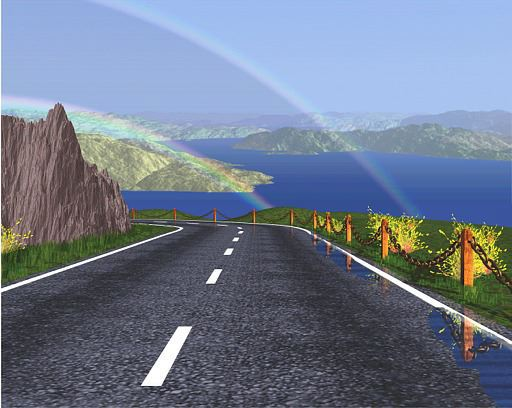
\includegraphics[width=0.7\textwidth]{./img/pointreyes.jpg}
    \caption{The Road to Point Reyes, rendered using the REYES algorithm.}
    \label{fig:reyes}
\end{figure}